\chapter{METHODOLOGY}
\label{ch:methodology}

This chapter describes how the system was built, in the order the work was carried out. The pipeline runs from establishing the signed form of each phrase with Deaf experts, through recording and preprocessing a custom dataset, to training the classifier, evaluating it, and deploying it. The evaluation protocol and the deployment path are described at the end, since both differ from what the proposal anticipated.

\section{Software Development Approach}

Agile incremental development was adopted because several parameters could not be fixed in advance. The sequence length depended on how long signers actually took to perform each phrase, the normalisation scheme had to be validated against real recordings, and the deployment target changed once the recognition results were in hand. Each increment delivered a working module: phrase verification, the recorder, the preprocessing core, the trained model, the inference server, and the mobile client.

The riskiest unknown was addressed first. Before any large-scale recording, a small set of clips was captured to confirm that MediaPipe Holistic produces stable landmarks for multi-sign NSL phrases performed at natural speed. Had it not, the entire landmark-based approach would have needed reconsideration while there was still time to change it.

\begin{figure}[H]
    \centering
    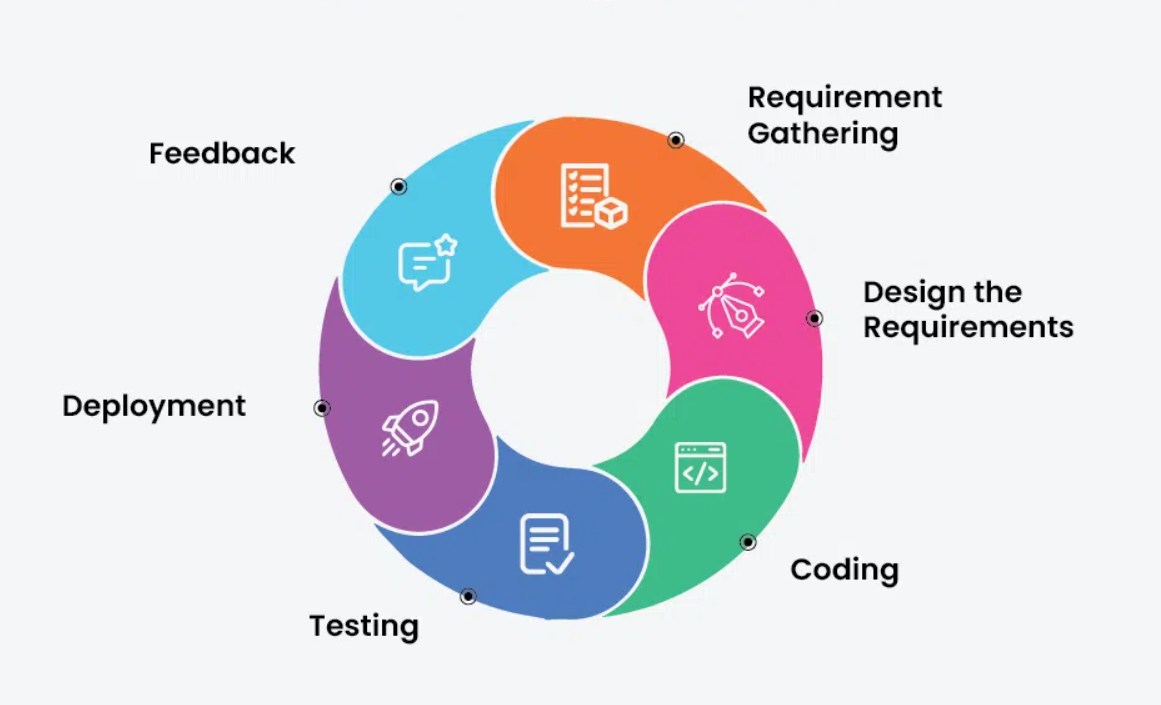
\includegraphics[width=0.7\textwidth]{img/sdlc.png}
    \caption{Agile incremental development approach}
    \label{fig:agile}
\end{figure}

\section{Phase 0: Establishing the Signed Form of Each Phrase}
\label{sec:phase0}

No standard published gloss exists for the six target emergency phrases, so the natural signed form of each had to be established with the Deaf community before recording could begin. Two consultations were held in person: with Yojana Sakha and colleagues at the Rehabilitation Centre for the Rural Deaf in Bhaktapur, and with a resource person at the National Federation of the Deaf Nepal in Ranibari Marga, Samakhushi, Kathmandu.

Each consultant was asked to demonstrate how the idea would be signed in an actual emergency, as concisely as possible, and not to sign the English sentence word by word. Each demonstration was discussed for regional variation, recorded as a reference, and confirmed as the form every signer would reproduce. Because the experts' time was limited, they also contributed roughly ten clips per phrase, which anchor the dataset to an authentic performance. Photographs from the consultations appear in Appendix~\ref{app:fieldwork}.

The consultants were also asked directly whether facial expression changes or adds meaning for any of the six phrases. They confirmed it does not for this phrase set, which settled the exclusion of the 468 face landmarks from the feature vector.

Table~\ref{tab:phrases} lists the six phrases and the situation each covers. Phrase 6 replaced an earthquake phrase considered at proposal stage. The consultants advised that a request to use the toilet is a far more frequent communication failure for deaf people in institutional settings than an earthquake report, and the change was approved at the mid-term defence.

\begin{table}[H]
    \centering
    \caption{Target emergency phrases and their categories}
    \label{tab:phrases}
    \small
    \begin{tabular}{|c|p{3.6cm}|p{3.4cm}|l|l|}
        \hline
        \textbf{\#} & \textbf{English phrase} & \textbf{Nepali phrase} & \textbf{Category} & \textbf{Class key} \\
        \hline
        1 & I can't breathe            & \nepali{मलाई सास फेर्न गाह्रो भइरहेको छ} & Medical           & \texttt{cant\_breathe} \\
        \hline
        2 & The building is on fire    & \nepali{भवनमा आगो लागेको छ} & Fire              & \texttt{building\_on\_fire} \\
        \hline
        3 & Call the police            & \nepali{प्रहरीलाई फोन गर्नुहोस्} & Crime             & \texttt{call\_police} \\
        \hline
        4 & I need an ambulance        & \nepali{मलाई एम्बुलेन्स चाहियो} & Medical           & \texttt{need\_ambulance} \\
        \hline
        5 & Help me / I am in danger   & \nepali{मलाई मद्दत गर्नुहोस् / म खतरामा छु} & Generic emergency & \texttt{help\_danger} \\
        \hline
        6 & I need to go to the toilet & \nepali{मलाई शौचालय जानु छ} & Basic need        & \texttt{need\_toilet} \\
        \hline
        7 & Not one of the above       & --- & Negative class    & \texttt{none} \\
        \hline
    \end{tabular}
\end{table}

\subsection{The Negative Class}

The seventh class was added during development and is not in the original proposal. A classifier over six phrases assigns one of those six to every input it receives, so a signer adjusting their glasses would be reported as an emergency. For a system whose output is a spoken emergency announcement, that is the worst available failure mode.

The \texttt{none} class holds deliberate non-examples: resting, idle movement, gestures outside the target set, and partial or abandoned signs. Giving the model explicit negatives lets it learn a decision boundary around the six real phrases instead of partitioning the whole input space among them, so the confidence threshold of Section~\ref{sec:decisionrule} has a class to fall back on instead of being forced to choose one of six emergency phrases for every input.

\section{Phase 1: Dataset Collection}

Because no public dataset of NSL emergency phrases exists, one was recorded from scratch. This was the most consequential phase of the project: the ceiling on recognition accuracy is set by the quality and variety of the recordings.

\subsection{The Recorder Application}

A purpose-built recorder was written for the task. It runs MediaPipe Holistic live on a webcam feed and, for every frame, extracts a 225-value vector: 33 pose landmarks, 21 left-hand landmarks, and 21 right-hand landmarks, each with $x$, $y$, and $z$ coordinates. The operator selects a signer identity and a phrase, then starts and stops each recording explicitly, so every clip corresponds to one deliberate performance of one phrase.

Every frame is mirrored horizontally before detection. This is recorded here because it is a constraint on everything downstream: the landmarks in the dataset describe a mirrored image, and any inference path that does not reproduce the same flip will present the model with the signer's hands swapped. Screenshots of the recorder in use appear in Appendix~\ref{app:recorder}.

Frames in which a hand or the pose is not detected are zero-filled for that block and the detection rate is recorded. The frame is not dropped. Each clip is therefore accompanied by a JSON sidecar holding its frame count, duration, and per-block detection rates, which made it possible to identify weak recordings without replaying them.

\subsection{Recording Setup and Variation}

Variation was introduced deliberately so the model would not learn a single recording condition:

\begin{itemize}
    \item Lighting: bright, dim, and mixed daylight near a window.
    \item Background: plain wall, cluttered room, and several different rooms.
    \item Distance: close to the camera and at arm's length or further.
    \item Signers: eight people, differing in body size, hand size, and signing speed.
    \item Speed: each signer performed each phrase somewhat faster and somewhat slower across takes.
\end{itemize}

Each clip is saved as \texttt{<phrase>\_\_<signer>\_\_<index>.npy}. Encoding the signer in the filename is what makes signer-independent evaluation possible later, and it was the reason for adopting the convention.

\subsection{Storing Landmarks Instead of Video}

The recorder saves only the per-frame landmark vectors. Video is never written to disk. This keeps the dataset small, removes a slow reprocessing step from every later stage, and means no video of any signer is stored or transmitted.

The cost is worth stating plainly. Because no video was kept, the landmark representation cannot be recomputed. Changing the landmark source, for example to run detection on a phone instead of a server, cannot be evaluated against the existing data and would require re-recording every clip.

\subsection{Aggregation Across Signers}

The eight signers recorded independently on separate machines. Git was used to merge each contribution into one shared repository instead of copying files by hand, which gave a reviewable history of what each signer added and caught duplicate and misnamed clips before they entered the combined set. Screenshots of the merged repository and the resulting directory layout appear in Appendix~\ref{app:dataorg}.

After aggregation the dataset held 840 clips: exactly 120 in each of the seven classes, contributed by eight signers. The composition is reported in full in Section~\ref{sec:datasetcomposition}.

\section{Phase 2: Feature Extraction}

Every frame of every clip is reduced to the same 225-dimensional vector, concatenated in a fixed order:

\begin{itemize}
    \item 33 pose landmarks $\times\ (x, y, z)$ = 99 values, at indices 0 to 98.
    \item 21 left-hand landmarks $\times\ (x, y, z)$ = 63 values, at indices 99 to 161.
    \item 21 right-hand landmarks $\times\ (x, y, z)$ = 63 values, at indices 162 to 224.
\end{itemize}

\noindent A clip is therefore a $(n_{\text{frames}}, 225)$ array of 32-bit floats, with $n_{\text{frames}}$ varying between clips. This layout, the normalisation anchors, and the sequence length are held as constants in a single module that both the training code and the inference server import, so the two cannot drift apart.

\section{Phase 3: Determining the Sequence Length}

The classifier requires a fixed number of time steps, but raw clip lengths vary because signers take different amounts of time. The value was measured from the data rather than chosen.

Across the 840 clips, frame counts ranged from 18 to 217, with a median of 89 and a mean of 90.1. The 95th percentile of this distribution gives $\textsc{seq\_len} = 137$ frames. The distribution and the cutoff are shown in Figure~\ref{fig:seqlen} in Chapter~\ref{ch:results}. The value is written to a metadata file that every later stage reads, so no stage recomputes or assumes it.

An observation from the same metadata turned out to matter more than expected. The recorder never locked a frame rate; it ran as fast as the interface and MediaPipe allowed, giving a median capture rate of 15.7 frames per second across a range of 10.8 to 21.2. Since the model receives a fixed-length sequence with no explicit time axis, it reads frame count as duration. The capture rate is therefore a property of the training data that any real-time path has to reproduce, and Section~\ref{sec:framerate} describes how.

\section{Phase 4: Normalisation and Standardisation}

Each clip is normalised and then standardised to \textsc{seq\_len}, in that order.

Normalisation applies the dual-anchor scheme of Section~\ref{sec:normalisation} to each frame, treating the three landmark blocks independently. The pose block is re-centred on the shoulder midpoint and divided by shoulder width; each hand block is re-centred on its wrist and divided by the wrist-to-middle-knuckle distance. Normalising per block keeps the position of a hand relative to the body while removing the signer's position and distance from the camera.

Standardisation then forces the clip to exactly 137 frames in one of three ways. A clip already at 137 frames is used unchanged. A longer clip is subsampled at 137 evenly spaced positions spanning its full duration, so the whole performance is represented instead of the first 137 frames. A shorter clip is zero-padded at the end, and a boolean mask records which frames are real.

The order is what makes the padding safe. Both normalisation formulas map a zero input to zero output, so an undetected block stays zero through normalisation, and padding added afterwards is also exactly zero. The classifier's masking layer then skips any all-zero time step at no cost. Padding after normalising would have produced non-zero padded frames that the model would read as signal.

The compiled dataset is stored as three aligned arrays: the normalised sequences with shape $(840, 137, 225)$, the integer labels with shape $(840,)$, and the padding mask with shape $(840, 137)$. A manifest records the class, signer, source file, and original frame count for every row, which keeps each compiled clip traceable to the recording it came from.

\section{Phase 5: Model Training}

\subsection{Architecture}

The classifier is a bidirectional LSTM built with TensorFlow and Keras:

\begin{table}[H]
    \centering
    \caption{Classifier architecture}
    \label{tab:architecture}
    \begin{tabular}{|l|l|}
        \hline
        \textbf{Layer} & \textbf{Purpose} \\
        \hline
        Input $(137, 225)$              & one normalised clip \\
        \hline
        Masking (mask value 0.0)        & skips zero-padded and undetected frames \\
        \hline
        Bidirectional LSTM, 64 units    & reads the motion in both directions \\
        \hline
        Dropout 0.3                     & regularisation \cite{srivastava2014dropout} \\
        \hline
        Bidirectional LSTM, 32 units    & summarises the sequence \\
        \hline
        Dropout 0.3                     & regularisation \\
        \hline
        Dense 32, ReLU                  & feature layer feeding the classification head \\
        \hline
        Dense 7, softmax                & probability over the seven classes \\
        \hline
    \end{tabular}
\end{table}

\noindent The network has 192{,}007 trainable parameters, which is small enough to train on a laptop CPU in minutes.

\subsection{Why This Model and Not a Larger Pretrained One}

A dataset of 840 clips is small for a network trained from scratch, which raises the
question of whether a pretrained model should carry more of the work. The answer is that
one already does, and that the division of labour is where the data efficiency comes from.

MediaPipe Holistic is the pretrained component. It was trained on far more human pose and
hand data than this project could ever collect, and it performs the part of the task that
needs that scale: locating a body and two hands in an arbitrary image under arbitrary
lighting. What reaches the BiLSTM is not an image but 225 already-interpreted coordinates,
so the only thing left to learn is how those coordinates move over time for each phrase.
That is a much smaller problem, and 192{,}007 parameters is a proportionate model for it.

A pretrained video classifier operating on pixels was considered and rejected for two
reasons. It would need the raw video, which was deliberately never stored, so adopting one
would mean re-recording the entire dataset. It would also be too large for the deployment
target, where the whole exported model is 879 kilobytes and runs without a GPU.

The dataset was also enlarged during development in preference to adding model capacity,
growing from four signers and 570 clips at the mid-term to eight signers and 840 clips.
For a landmark-based classifier at this vocabulary size, additional signers buy more than
additional parameters, because the quantity in short supply is variation between people and
not model expressiveness.

\subsection{Training Configuration}

Training minimises sparse categorical cross-entropy with the Adam optimiser \cite{kingma2015adam} at a batch size of 16, for at most 200 epochs. Class weights are computed to be inversely proportional to class frequency, which matters more for the folds than for the whole dataset, since the classes are balanced overall but a held-out signer's contribution is not always uniform.

Two callbacks control the schedule. Early stopping monitors validation loss with a patience of 15 epochs and restores the best weights. Its minimum-improvement threshold is set to $10^{-3}$ and not left at zero, because with a threshold of zero any improvement at all resets the patience counter, including a change in the fourth decimal place. Once validation loss approaches zero it keeps setting negligible new records, so training does not end on convergence; it ends whenever an optimiser instability finally breaks the streak. That made the epoch count a record of when a random fluctuation occurred instead of a property of the fit.

Learning rate reduction on plateau addresses the cause of those fluctuations, halving the learning rate after 6 epochs without improvement, down to a floor of $10^{-5}$. Its patience is kept well below the early-stopping patience so that the reduced rate has a chance to take effect before training halts.

Reproducibility required more than fixing the random seed. TensorFlow's parallel CPU reductions vary between runs, and on identical data this moved per-fold accuracy by up to 2.7 percentage points. Deterministic operations are therefore enabled explicitly, at some cost in speed, so that a reported fold accuracy is a property of the data and the recipe, not of one particular run.

\section{Phase 6: Evaluation Methodology}

\subsection{Leave-One-Signer-Out}

The headline metric is leave-one-signer-out accuracy. For each signer eligible to be held out, the model is trained from scratch on every clip from the other signers and tested only on that signer's clips. Within each fold, 15\% of the training clips are set aside as a stratified validation split for early stopping, so the held-out signer influences neither the fitted weights nor the stopping point.

A signer is eligible for holdout only if removing their clips leaves every class present in the remainder. All eight signers satisfied this, giving eight folds. Two figures are reported: the mean accuracy across folds, which estimates performance on a new person, and the pooled accuracy over all 840 predictions, where each clip is scored exactly once by a model that never saw its signer.

\subsection{The Random-Split Contrast}

A stratified 70/15/15 random split is also trained and reported. It is not an additional performance measure. Its purpose is to quantify what the signer-independent protocol is protecting against: under a random split, clips from the same person appear in both training and test, and the model can score well by recognising individuals. The gap between the two protocols is the size of that effect on this dataset, and it is discussed in Section~\ref{sec:leakage}.

\subsection{Metrics}

Overall accuracy is reported alongside per-class precision, recall, and F1:
\begin{equation}
    \text{Precision} = \frac{TP}{TP+FP}, \quad
    \text{Recall} = \frac{TP}{TP+FN}, \quad
    \text{F1} = \frac{2\,\text{Precision}\cdot\text{Recall}}{\text{Precision}+\text{Recall}}.
\end{equation}
A confusion matrix pooled over all folds identifies which classes are mutually confusable. For an emergency system the two directions of error are not equivalent: failing to recognise a real phrase leaves the user without help, while announcing a phrase for a non-sign produces a false alarm. Both appear in the matrix and are discussed separately.

\section{Phase 7: Deployment}

\subsection{Revision of the Deployment Approach}
\label{sec:deploychange}

The proposal specified a browser application built with Next.js, running the model in the visitor's browser through TensorFlow.js, with no server involved. The delivered system is an Android application that streams frames to an inference server. Two separate decisions produced that change and they are worth separating.

The first is the choice of device. A phone is what a person has with them when an emergency happens; a laptop with a browser open is not. For a tool whose value depends on being available at the moment of need, the phone is the correct target, and this was decided on those grounds. The browser route was not attempted. The change was recorded as a task deviation in the project log and accepted by the supervisor before the client was built.

The second decision concerns where inference runs, and it carries a real cost. MediaPipe Holistic, the exact landmark extractor the dataset was recorded with, exists as a Python pipeline. Running recognition on the device would mean reimplementing the 225-feature extraction and the dual-anchor normalisation against a different landmark source, and a numerical difference between the two implementations does not raise an error. It produces confident wrong answers, because the model receives numbers unlike anything it was trained on. Serving from Python means the inference path imports the same preprocessing module that the reported accuracy was measured with, so the correspondence between measured and deployed behaviour is structural, not something that had to be verified.

The cost is that the delivered system requires a network connection at use time, which the proposal stated it would not. For an emergency tool this is a genuine weakness and not a neutral trade. It is listed among the limitations in Chapter~\ref{ch:conclusion}, along with the work that would remove it.

\subsection{Model Export}

The trained model is converted to TensorFlow Lite \cite{tflite2024} so the server can run it without a full TensorFlow installation, reducing the deployed image from about three gigabytes to one. The conversion required a workaround: on the pinned TensorFlow and Keras versions used here, the standard converter entry points abort the host process inside the compiler backend instead of raising a catchable exception. Freezing the model's variables to constants before conversion avoids the failure.

Because a silent conversion error would be indistinguishable from a model that simply performs worse, the export is verified and not assumed. The converted model and the original are run on 30 real clips and compared; the export is rejected if they disagree. The measured agreement is reported in Section~\ref{sec:exportverify}.

\subsection{Inference Server}

The server is a FastAPI application exposing a WebSocket endpoint. A client opens a session, streams JPEG frames while the user signs, and sends a completion message; the server replies with the decision. Landmark extraction costs about 38 milliseconds per frame and accounts for almost the entire pipeline cost, so streaming frames during signing overlaps that work with the signing itself. When the client signals completion, only normalisation, standardisation, and the forward pass remain, which together take about 15 milliseconds. Uploading a finished recording instead would have serialised the two and added several seconds of silence before every result.

Each session holds its own MediaPipe graph, which occupies about 150 megabytes, so concurrency is bounded by memory, not processor time. A semaphore caps simultaneous sessions and refuses further connections with an explicit error instead of allowing the process to be killed for exhausting memory. Requests are authenticated with a shared key compared using a constant-time function, so that a wrong key cannot be narrowed down by timing the response. The health endpoint is left unauthenticated so that container health checks and the client's reachability test continue to work.

\subsection{Frame Rate as a Correctness Constraint}
\label{sec:framerate}

Because the model reads frame count as duration, a client capturing at 30 frames per second produces twice as many frames for the same sign as the training data contained, and presents the model with a temporal scale it has never seen. The server therefore discards incoming frames down to the 15.7 frames per second of the training data before running detection, using an accumulator that tracks when the next frame is due. A simpler test of whether enough time has elapsed since the last accepted frame aliases a 16 frames-per-second client down to 8. The client caps its own send rate at 16 frames per second, slightly above the target so that jitter does not starve the server below it.

\subsection{Mobile Client}

The Android client performs no recognition. It captures camera frames, encodes them, sends them, and speaks the result.

Frame encoding is the client's bottleneck, since it is pure Dart. Colour conversion, rotation, and downscaling are folded into a single pass over the output pixels, avoiding the intermediate full-resolution buffers a naive implementation allocates. Frames are downscaled to 320 pixels wide and encoded with chroma subsampling, on the grounds that landmarks are derived from luminance structure and not chroma resolution. The work runs on a persistent background isolate. When a frame is already in flight the next one is dropped instead of queued, since the server discards surplus frames anyway and a queue would only add latency.

Two details are recorded because they are easy to get wrong. The application is locked to portrait orientation and rotates each frame by the camera's sensor orientation before sending, because Android delivers frames in sensor orientation and MediaPipe detects nothing at all in an image of a person lying sideways. Frames are sent unmirrored with a flag instructing the server to apply the same horizontal flip the recorder used, and the flag is set for both front and rear cameras: the lens faces the signer either way, so the signer's right hand appears on the image-left in both cases, and making the flag depend on the camera would swap the two hand blocks in the feature vector for one of them.

\subsection{The Decision Rule}
\label{sec:decisionrule}

Two outcomes are possible:

\begin{enumerate}
    \item If the predicted class is one of the six emergency phrases and the softmax confidence reaches 0.75, the result is \texttt{accepted}. The phrase is displayed and spoken.
    \item Otherwise the result is \texttt{low\_confidence}. This covers a prediction of the \texttt{none} class and a low-confidence prediction of any class alike: the user is told the input was not recognised clearly, and nothing is spoken.
\end{enumerate}

\noindent Folding rejection into the classifier this way keeps a wrong announcement and no announcement on the same footing: both routes into \texttt{low\_confidence} withhold output rather than guessing. The best guess and the top three probabilities are returned in every case, including refusals, which is what makes a failure diagnosable during a demonstration.
